\part{框架与分工}

\section{整体框架}

本次编程实验的整体框架如下图所示。主要任务包括电平映射模块的设计,卷积码编解码模块的设计,CRC模块的设计,以及针对具体传输任务的编码方案设计。

\begin{figure}[h]
    \centering
    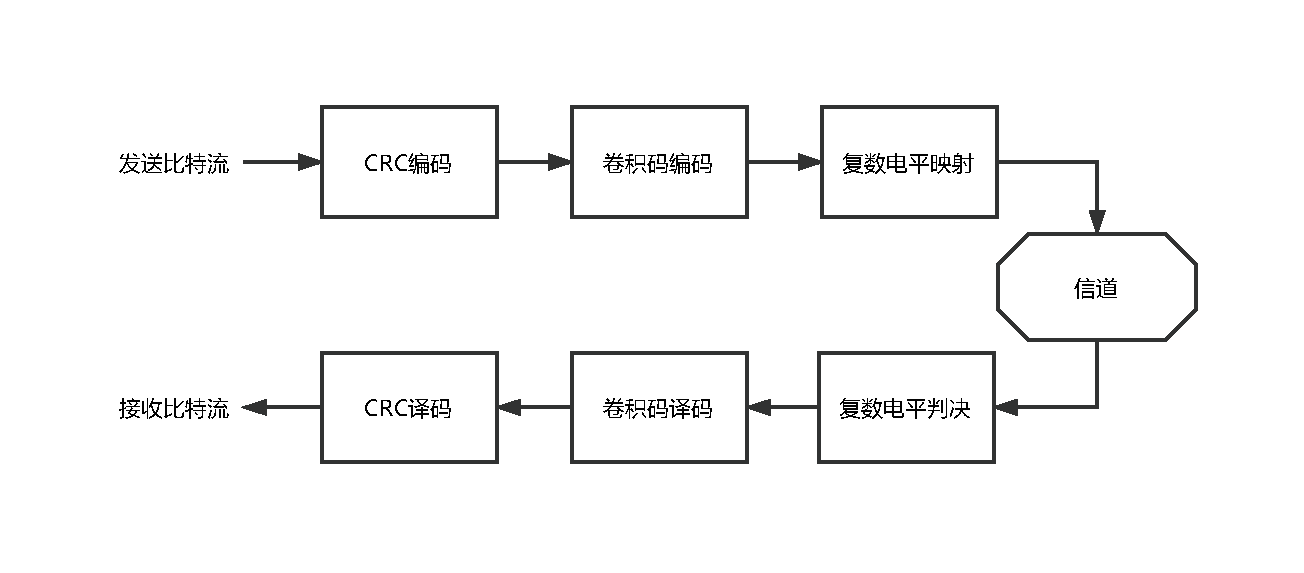
\includegraphics[width=0.9\textwidth,trim=0 40 0 40,clip]{pic/framework.eps}
    \caption{整体设计框架图}
\end{figure}

\section{分工情况}

\paragraph{邓程昊}
\indent

\begin{itemize}
    \item 场景二下ASK的设计、推导、实现、仿真;
    \item 不同情况下卷积码编译码的仿真、比较、分析;
    \item 场景二下具体方案的最佳设计。
\end{itemize}

\paragraph{齐涛}
\indent

\begin{itemize}
    \item 场景一下PHIMAP算法的设计、推导、实现、仿真,以及和BMPSK的对比、分析;
    \item CRC模块的实现、误块率和误码图案的统计;
    \item 场景一下具体方案的最佳设计。
\end{itemize}

\paragraph{徐泽来}
\indent

\begin{itemize}
    \item 场景一下BMPSK映射的设计、推导、实现、仿真、折衷;
    \item 卷积码编译码的编码、硬判决、软判决、仿真。	
\end{itemize}	

\paragraph{说明}
\indent

综合考虑讨论、设计、实现、仿真、分析、报告各个部分的情况,我们认为我们小组基本是均匀分配的工作量。
